\documentclass[12pt,a4paper]{article}
\usepackage[utf8]{inputenc}
\usepackage[english]{babel}
\usepackage{geometry}
\usepackage{fancyhdr}
\usepackage{graphicx}
\usepackage{longtable}
\usepackage{array}
\usepackage{booktabs}
\usepackage{xcolor}
\usepackage{hyperref}
\usepackage{listings}
\usepackage{enumitem}
\usepackage{caption}
\usepackage{float} % for [H] placement
\geometry{margin=1in}
\pagestyle{fancy}
\fancyhf{}
\rhead{\thepage}
\lhead{HIV Clinic RDS}
\setlength{\headheight}{14.5pt}

\title{\textbf{Requirement \& Design Specification\\HIV Clinic Appointment Booking System}}
\author{Version: 2.0}
\date{January 2025}

\begin{document}

\maketitle

\newpage

\tableofcontents

\newpage

\section{Introduction}

\subsection{Purpose}
This Requirements Design Specification (RDS) document provides a comprehensive specification for the HIV Clinic Management System. This system is designed to streamline appointment booking, patient management, and HIV treatment monitoring processes for both healthcare providers and patients.

\subsection{Scope}
The HIV Clinic Management System encompasses:
\begin{itemize}
    \item User authentication and role-based access control
    \item Patient and doctor management
    \item Appointment booking and scheduling
    \item Medical record management with HIV-specific features
    \item ARV (Antiretroviral) treatment tracking and monitoring
    \item Notification and reminder systems
    \item Administrative dashboards and reporting
\end{itemize}

\subsection{Document Structure}
This document follows the template structure and contains:
\begin{itemize}
    \item Requirements Specifications with use case mappings
    \item Comprehensive Use Case Specifications for all 27 use cases
    \item Detailed Design Specifications for all system components
    \item Technical appendices and supporting documentation
\end{itemize}

\subsection{Stakeholders}
\begin{itemize}
    \item \textbf{Patients}: Individuals seeking HIV care and treatment
    \item \textbf{Doctors}: Healthcare providers treating HIV patients
    \item \textbf{Administrators}: System administrators managing clinic operations
    \item \textbf{Managers}: Clinic managers overseeing operations and analytics
    \item \textbf{IT Staff}: Technical personnel maintaining the system
\end{itemize}

\newpage

\section{Requirements Specifications}

\subsection{Functional Requirements Overview}

The system implements 27 distinct use cases organized by functional areas:

\begin{longtable}{|c|c|c|p{8.5cm}|}
\hline
\textbf{\#} & \textbf{Feature} & \textbf{Screen} & \textbf{Description} \\
\hline
\endfirsthead

\hline
\textbf{\#} & \textbf{Feature} & \textbf{Screen} & \textbf{Description} \\
\hline
\endhead

1 & Public Access & Home Page & Browse public HIV information and educational content \\
\hline
2 & Authentication & Register Page & User registration for patients and doctors \\
\hline
3 & Authentication & Login Page & Secure user authentication with role-based routing \\
\hline
4 & Dashboard & Patient Dashboard & Personalized patient interface \\
\hline
5 & Profile & Profile Management & Update personal profile information \\
\hline
6 & Security & Password Management & Change user passwords securely \\
\hline
7 & Dashboard & Dashboard View & Role-based dashboard access \\
\hline
8 & Appointments & Appointment Management & Book, view, and cancel appointments \\
\hline
9 & Medical Records & Personal Records & Manage personal medical records \\
\hline
10 & Notifications & Notification Center & View system notifications \\
\hline
11 & Authentication & Logout & Secure session termination \\
\hline
12 & Dashboard & Doctor Dashboard & Professional doctor interface \\
\hline
13 & Appointments & Doctor Appointments & Manage doctor-side appointments \\
\hline
14 & Scheduling & Availability Slots & Manage doctor availability \\
\hline
15 & Medical Records & Patient Records Access & Access patient medical records \\
\hline
16 & Treatment & ARV Management & Manage HIV antiretroviral treatments \\
\hline
17 & Communications & Patient Notifications & Send notifications to patients \\
\hline
18 & Dashboard & Admin Dashboard & Administrative system overview \\
\hline
19 & User Management & User Administration & Manage system users \\
\hline
20 & Monitoring & Appointment Oversight & View all system appointments \\
\hline
21 & Content Management & Blog Management & Manage educational blog content \\
\hline
22 & Dashboard & Manager Dashboard & Operational management interface \\
\hline
23 & Administration & Patient Records Admin & Administrative patient record management \\
\hline
24 & Administration & Doctor Records Admin & Administrative doctor record management \\
\hline
25 & Analytics & System Analytics & Comprehensive system analytics \\
\hline
26 & Reporting & Data Export & Export system data for analysis \\
\hline
27 & Analytics & Clinic Statistics & View clinic operational statistics \\
\hline
\end{longtable}

\subsection{Use Case Diagram}

\begin{figure}[H]
\centering
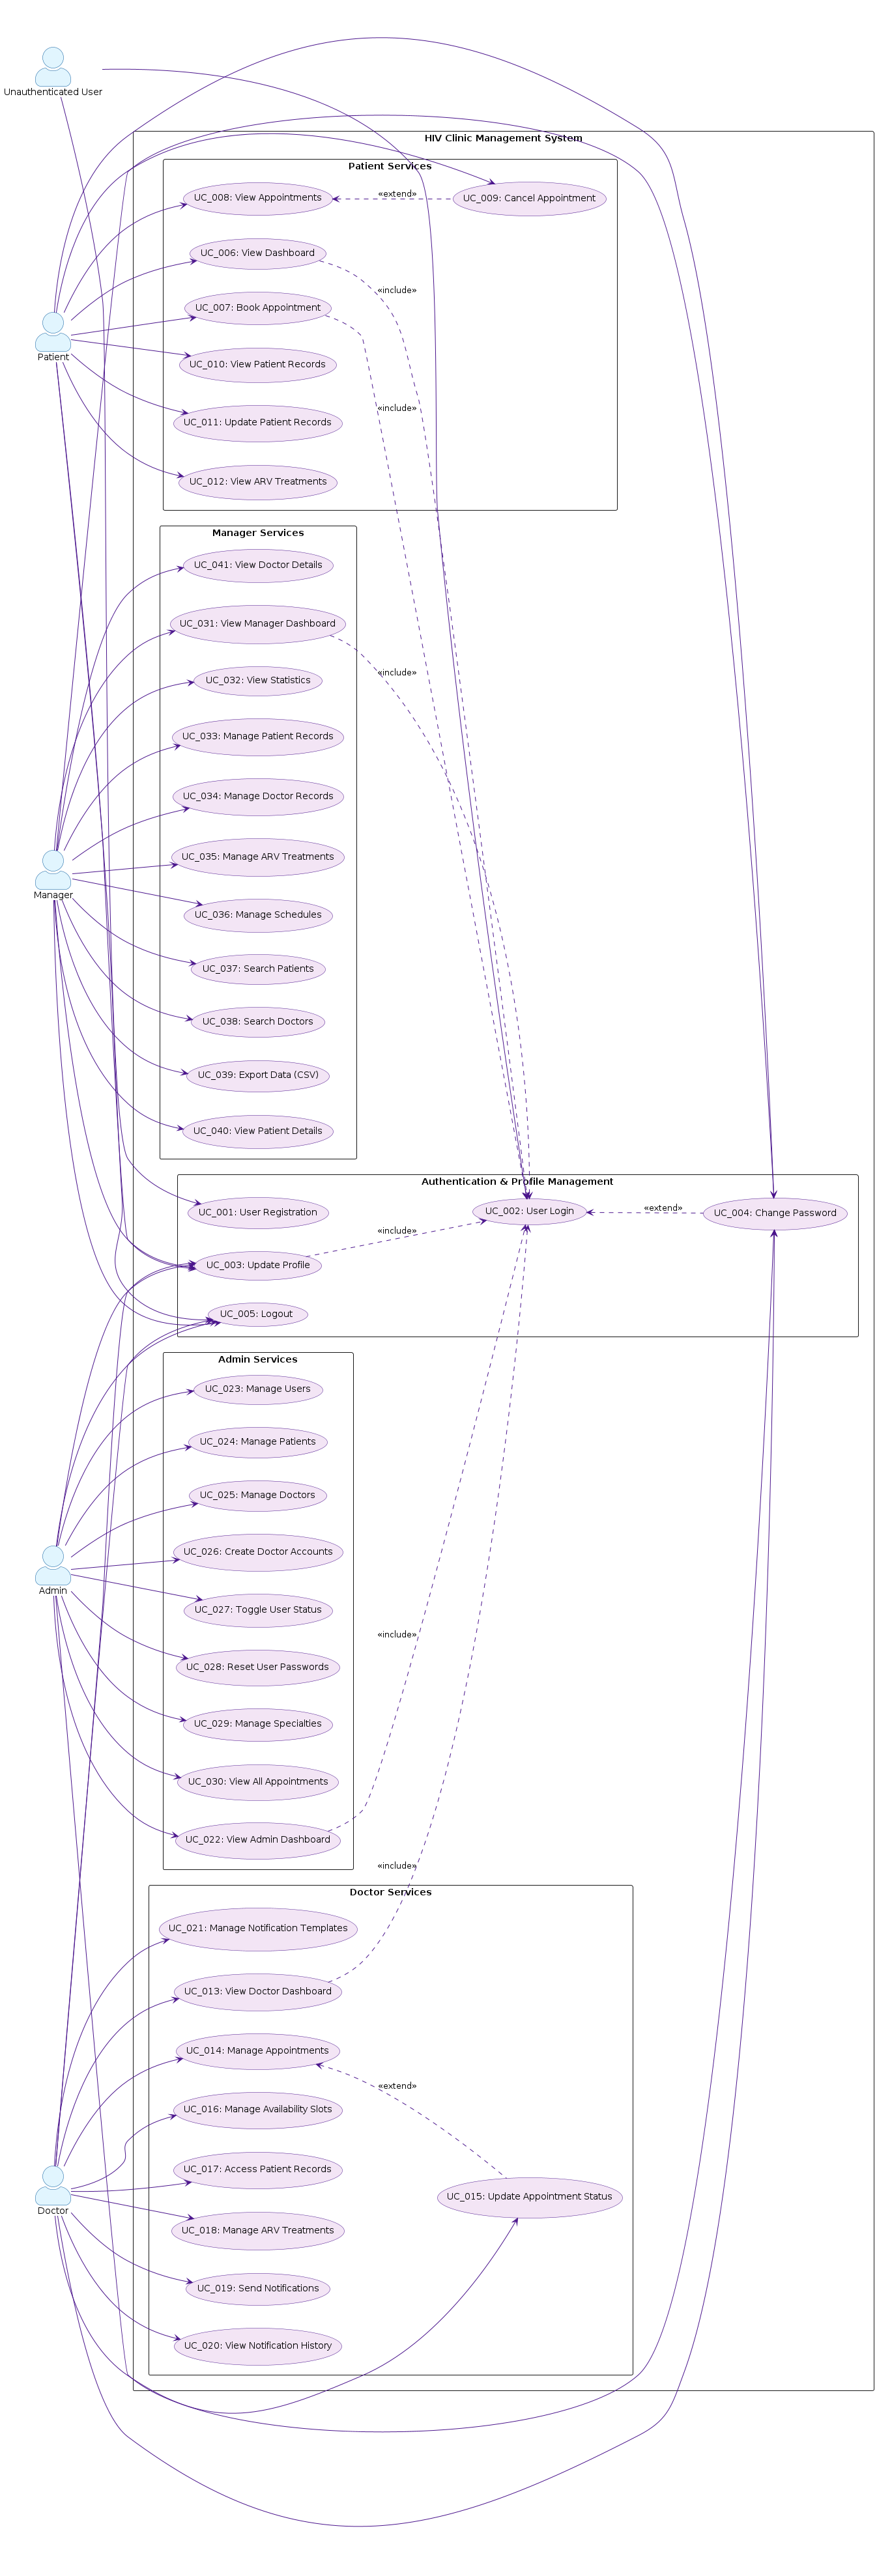
\includegraphics[width=0.9\textwidth]{diagrams/use_case_diagram.png}
\caption{HIV Clinic Management System Use Case Diagram}
\label{fig:use-case-diagram}
\end{figure}

The use case diagram shows the complete system with 27 use cases, two primary actors (Unauthenticated User and Authenticated User), and proper UML relationships including associations, generalizations, includes, and extends.

\subsection{User Interface Flow}

\begin{figure}[H]
    \centering
    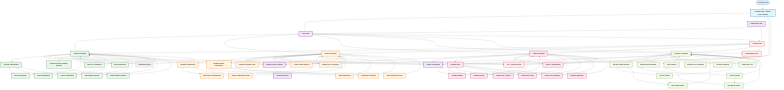
\includegraphics[width=0.9\textwidth]{diagrams/user_interface_flow.png}
    \caption{Overall Screen Flow}
    \label{fig:screen-flow}
\end{figure}

The interface flow demonstrates role-based navigation from public access through authentication to specialized dashboards for different user types.

\newpage

\section{Use Case Specifications}

\subsection{UC-001 – Browse Public Website}

\renewcommand{\arraystretch}{1.5}
\begin{longtable}{|p{4.5cm}|p{10.5cm}|}
\hline
\textbf{UC ID and Name:} & UC-001 – Browse Public Website \\
\hline
\textbf{Created By:} & System Analyst \\
\hline
\textbf{Date Created:} & January 2025 \\
\hline
\textbf{Primary Actor:} & Unauthenticated User \\
\hline
\textbf{Secondary Actors:} & None \\
\hline
\textbf{Description:} & Users can view HIV information, educational content, and blog posts without requiring authentication \\
\hline
\textbf{Trigger:} & User accesses the website homepage or navigation menu \\
\hline
\textbf{Preconditions:} &
\begin{itemize}
  \item The system is online and accessible
  \item Public content is available in the system
\end{itemize} \\
\hline
\textbf{Postconditions:} &
\begin{itemize}
  \item Public HIV information and content is displayed
  \item User can navigate through available public pages
\end{itemize} \\
\hline
\textbf{Normal Flow:} &
\begin{enumerate}
  \item User opens the website
  \item System displays homepage with HIV clinic information
  \item User navigates through public content sections
  \item User can read educational content and blog posts
\end{enumerate} \\
\hline
\textbf{Alternative Flows:} & 
\textbf{AF-1:} User accesses specific public pages directly via URL \\
\hline
\textbf{Exceptions:} &
\begin{itemize}
  \item EX-1: If public content is unavailable, system displays maintenance message
\end{itemize} \\
\hline
\textbf{Business Rules:} &
\begin{itemize}
  \item BR-001: Public content must be accessible without authentication
  \item BR-002: HIV educational content must be medically accurate
\end{itemize} \\
\hline
\textbf{Priority:} & High \\
\hline
\textbf{Frequency of Use:} & High \\
\hline
\end{longtable}

\subsection{UC-002 – User Registration}

\renewcommand{\arraystretch}{1.5}
\begin{longtable}{|p{4.5cm}|p{10.5cm}|}
\hline
\textbf{UC ID and Name:} & UC-002 – User Registration \\
\hline
\textbf{Created By:} & System Analyst \\
\hline
\textbf{Date Created:} & January 2025 \\
\hline
\textbf{Primary Actor:} & Unauthenticated User \\
\hline
\textbf{Secondary Actors:} & System \\
\hline
\textbf{Description:} & New users (patients and doctors) can create accounts with role-based access to the HIV clinic system \\
\hline
\textbf{Trigger:} & User clicks "Register" from homepage or login page \\
\hline
\textbf{Preconditions:} &
\begin{itemize}
  \item User is not currently logged in
  \item Registration system is operational
\end{itemize} \\
\hline
\textbf{Postconditions:} &
\begin{itemize}
  \item New user account is created in the system
  \item User receives confirmation notification
  \item User can login with new credentials
\end{itemize} \\
\hline
\textbf{Normal Flow:} &
\begin{enumerate}
  \item User accesses registration form
  \item User provides required information (name, email, phone, role)
  \item User creates username and password
  \item System validates input data
  \item System creates new user account
  \item System sends confirmation notification
\end{enumerate} \\
\hline
\textbf{Alternative Flows:} &
\textbf{AF-1:} Email already exists → System shows error and suggests login \\
\textbf{AF-2:} Invalid data format → System highlights errors for correction \\
\hline
\textbf{Exceptions:} &
\begin{itemize}
  \item EX-1: System error during registration → Show error message and retry option
\end{itemize} \\
\hline
\textbf{Business Rules:} &
\begin{itemize}
  \item BR-003: Email addresses must be unique in the system
  \item BR-004: Passwords must meet security requirements
  \item BR-005: Doctor registrations require additional verification
\end{itemize} \\
\hline
\textbf{Priority:} & High \\
\hline
\textbf{Frequency of Use:} & Medium \\
\hline
\end{longtable}

\subsection{UC-003 – User Login}

\renewcommand{\arraystretch}{1.5}
\begin{longtable}{|p{4.5cm}|p{10.5cm}|}
\hline
\textbf{UC ID and Name:} & UC-003 – User Login \\
\hline
\textbf{Created By:} & System Analyst \\
\hline
\textbf{Date Created:} & January 2025 \\
\hline
\textbf{Primary Actor:} & Unauthenticated User \\
\hline
\textbf{Secondary Actors:} & System \\
\hline
\textbf{Description:} & Existing users authenticate using username/password with JWT token-based security \\
\hline
\textbf{Trigger:} & User accesses login page and submits credentials \\
\hline
\textbf{Preconditions:} &
\begin{itemize}
  \item A registered account exists
  \item The user is not currently logged in
  \item Authentication system is operational
\end{itemize} \\
\hline
\textbf{Postconditions:} &
\begin{itemize}
  \item The user is authenticated
  \item The user is redirected to their personal dashboard
  \item Login activity is logged for security
\end{itemize} \\
\hline
\textbf{Normal Flow:} &
\begin{enumerate}
  \item User enters username/email and password
  \item The system validates the credentials
  \item System generates JWT token
  \item User is redirected to appropriate dashboard based on role
  \item System logs successful login
\end{enumerate} \\
\hline
\textbf{Alternative Flows:} &
\textbf{AF-1:} Invalid credentials → System shows error message \\
\textbf{AF-2:} Account disabled → System shows account status message \\
\hline
\textbf{Exceptions:} &
\begin{itemize}
  \item EX-1: Multiple failed attempts → Account temporarily locked
  \item EX-2: System authentication error → Show retry option
\end{itemize} \\
\hline
\textbf{Business Rules:} &
\begin{itemize}
  \item BR-006: Maximum 3 failed login attempts before temporary account lockout
  \item BR-007: Session timeout after 2 hours of inactivity
  \item BR-008: All login attempts must be logged for security audit
\end{itemize} \\
\hline
\textbf{Priority:} & High \\
\hline
\textbf{Frequency of Use:} & High \\
\hline
\end{longtable}

\subsection{UC-004 – View Patient Dashboard}

\renewcommand{\arraystretch}{1.5}
\begin{longtable}{|p{4.5cm}|p{10.5cm}|}
\hline
\textbf{UC ID and Name:} & UC-004 – View Patient Dashboard \\
\hline
\textbf{Created By:} & System Analyst \\
\hline
\textbf{Date Created:} & January 2025 \\
\hline
\textbf{Primary Actor:} & Authenticated User (Patient) \\
\hline
\textbf{Secondary Actors:} & System \\
\hline
\textbf{Description:} & Patients access their personalized dashboard showing appointments, medical records, notifications, and treatment information \\
\hline
\textbf{Trigger:} & Patient successfully logs in or navigates to dashboard \\
\hline
\textbf{Preconditions:} &
\begin{itemize}
  \item Patient is authenticated and logged in
  \item Patient has appropriate access permissions
\end{itemize} \\
\hline
\textbf{Postconditions:} &
\begin{itemize}
  \item Dashboard displays current patient information
  \item Quick access to key patient functions is available
  \item Recent activity and notifications are shown
\end{itemize} \\
\hline
\textbf{Normal Flow:} &
\begin{enumerate}
  \item System verifies patient authentication
  \item System retrieves patient-specific data
  \item Dashboard displays upcoming appointments
  \item Dashboard shows recent medical activity
  \item Patient can access primary functions (appointments, records, notifications)
\end{enumerate} \\
\hline
\textbf{Alternative Flows:} &
\textbf{AF-1:} First-time login → System shows welcome tour \\
\textbf{AF-2:} No recent activity → Dashboard shows guidance for getting started \\
\hline
\textbf{Exceptions:} &
\begin{itemize}
  \item EX-1: Data loading error → Show error message with refresh option
  \item EX-2: Session expired → Redirect to login page
\end{itemize} \\
\hline
\textbf{Business Rules:} &
\begin{itemize}
  \item BR-009: Patients can only view their own information
  \item BR-010: Recent activity is limited to last 30 days
\end{itemize} \\
\hline
\textbf{Priority:} & High \\
\hline
\textbf{Frequency of Use:} & High \\
\hline
\end{longtable}

\subsection{UC-005 – Update Profile}

\renewcommand{\arraystretch}{1.5}
\begin{longtable}{|p{4.5cm}|p{10.5cm}|}
\hline
\textbf{UC ID and Name:} & UC-005 – Update Profile \\
\hline
\textbf{Created By:} & System Analyst \\
\hline
\textbf{Date Created:} & January 2025 \\
\hline
\textbf{Primary Actor:} & Authenticated User \\
\hline
\textbf{Secondary Actors:} & System \\
\hline
\textbf{Description:} & Users can update their personal profile information including contact details and preferences \\
\hline
\textbf{Trigger:} & User navigates to profile settings and initiates update \\
\hline
\textbf{Preconditions:} &
\begin{itemize}
  \item User is authenticated and logged in
  \item Profile data exists in the system
\end{itemize} \\
\hline
\textbf{Postconditions:} &
\begin{itemize}
  \item Profile information is updated in the system
  \item User receives confirmation of successful update
  \item Updated information is reflected across the system
\end{itemize} \\
\hline
\textbf{Normal Flow:} &
\begin{enumerate}
  \item User accesses profile settings
  \item System displays current profile information
  \item User modifies editable fields
  \item User submits updated information
  \item System validates and saves changes
  \item System confirms successful update
\end{enumerate} \\
\hline
\textbf{Alternative Flows:} &
\textbf{AF-1:} Invalid data → System highlights errors for correction \\
\textbf{AF-2:} No changes made → System displays "no changes detected" message \\
\hline
\textbf{Exceptions:} &
\begin{itemize}
  \item EX-1: Email already in use → Show error and suggest alternatives
  \item EX-2: Database error → Show error message and retry option
\end{itemize} \\
\hline
\textbf{Business Rules:} &
\begin{itemize}
  \item BR-011: Email addresses must remain unique
  \item BR-012: Certain fields (role, user ID) cannot be modified by users
  \item BR-013: Phone numbers must follow valid format
\end{itemize} \\
\hline
\textbf{Priority:} & Medium \\
\hline
\textbf{Frequency of Use:} & Low \\
\hline
\end{longtable}

\subsection{UC-006 – Change Password}

\renewcommand{\arraystretch}{1.5}
\begin{longtable}{|p{4.5cm}|p{10.5cm}|}
\hline
\textbf{UC ID and Name:} & UC-006 – Change Password \\
\hline
\textbf{Created By:} & System Analyst \\
\hline
\textbf{Date Created:} & January 2025 \\
\hline
\textbf{Primary Actor:} & Authenticated User \\
\hline
\textbf{Secondary Actors:} & System \\
\hline
\textbf{Description:} & Users can change their account password for security purposes \\
\hline
\textbf{Trigger:} & User accesses password change functionality \\
\hline
\textbf{Preconditions:} &
\begin{itemize}
  \item User is authenticated and logged in
  \item User knows current password
\end{itemize} \\
\hline
\textbf{Postconditions:} &
\begin{itemize}
  \item Password is updated in the system
  \item User receives confirmation of password change
  \item Password change is logged for security audit
\end{itemize} \\
\hline
\textbf{Normal Flow:} &
\begin{enumerate}
  \item User accesses password change form
  \item User enters current password
  \item User enters new password twice for confirmation
  \item System validates current password
  \item System validates new password meets requirements
  \item System updates password and logs activity
\end{enumerate} \\
\hline
\textbf{Alternative Flows:} &
\textbf{AF-1:} Current password incorrect → Show error message \\
\textbf{AF-2:} New passwords don't match → Highlight mismatch error \\
\hline
\textbf{Exceptions:} &
\begin{itemize}
  \item EX-1: New password doesn't meet requirements → Show specific requirements
  \item EX-2: System error → Show error message and retry option
\end{itemize} \\
\hline
\textbf{Business Rules:} &
\begin{itemize}
  \item BR-014: New password must meet security requirements
  \item BR-015: Cannot reuse last 3 passwords
  \item BR-016: Password changes must be logged for security
\end{itemize} \\
\hline
\textbf{Priority:} & High \\
\hline
\textbf{Frequency of Use:} & Low \\
\hline
\end{longtable}

\subsection{UC-007 – View Dashboard}

\renewcommand{\arraystretch}{1.5}
\begin{longtable}{|p{4.5cm}|p{10.5cm}|}
\hline
\textbf{UC ID and Name:} & UC-007 – View Dashboard \\
\hline
\textbf{Created By:} & System Analyst \\
\hline
\textbf{Date Created:} & January 2025 \\
\hline
\textbf{Primary Actor:} & Authenticated User \\
\hline
\textbf{Secondary Actors:} & System \\
\hline
\textbf{Description:} & Users access role-appropriate dashboards with personalized information and quick access to key functions \\
\hline
\textbf{Trigger:} & User navigates to dashboard after login or from navigation menu \\
\hline
\textbf{Preconditions:} &
\begin{itemize}
  \item User is authenticated and logged in
  \item User has appropriate role permissions
\end{itemize} \\
\hline
\textbf{Postconditions:} &
\begin{itemize}
  \item Role-appropriate dashboard is displayed
  \item User can access relevant system functions
  \item Recent activity and notifications are shown
\end{itemize} \\
\hline
\textbf{Normal Flow:} &
\begin{enumerate}
  \item System determines user role
  \item System loads role-specific dashboard layout
  \item Dashboard displays relevant widgets and information
  \item User can interact with dashboard elements
  \item User can navigate to detailed functions
\end{enumerate} \\
\hline
\textbf{Alternative Flows:} &
\textbf{AF-1:} Multiple roles → System shows role selector \\
\textbf{AF-2:} Dashboard customization → User can modify widget preferences \\
\hline
\textbf{Exceptions:} &
\begin{itemize}
  \item EX-1: Data loading error → Show error message with refresh option
  \item EX-2: Permission denied → Redirect to appropriate page
\end{itemize} \\
\hline
\textbf{Business Rules:} &
\begin{itemize}
  \item BR-017: Dashboard content must match user role permissions
  \item BR-018: Sensitive information requires additional verification
\end{itemize} \\
\hline
\textbf{Priority:} & High \\
\hline
\textbf{Frequency of Use:} & High \\
\hline
\end{longtable}

\subsection{UC-008 – Manage Appointments}

\renewcommand{\arraystretch}{1.5}
\begin{longtable}{|p{4.5cm}|p{10.5cm}|}
\hline
\textbf{UC ID and Name:} & UC-008 – Manage Appointments \\
\hline
\textbf{Created By:} & System Analyst \\
\hline
\textbf{Date Created:} & January 2025 \\
\hline
\textbf{Primary Actor:} & Patient \\
\hline
\textbf{Secondary Actors:} & System, Doctor \\
\hline
\textbf{Description:} & Patients can book, view, and cancel appointments with available doctors \\
\hline
\textbf{Trigger:} & Patient accesses appointment management section \\
\hline
\textbf{Preconditions:} &
\begin{itemize}
  \item Patient is logged in to the system
  \item At least one doctor has available appointment slots
\end{itemize} \\
\hline
\textbf{Postconditions:} &
\begin{itemize}
  \item Appointment is successfully booked, viewed, or cancelled
  \item Doctor and patient receive appropriate notifications
  \item Appointment status is updated in the system
\end{itemize} \\
\hline
\textbf{Normal Flow:} &
\textbf{Booking:}
\begin{enumerate}
  \item Patient selects doctor from available list
  \item Patient chooses available date and time slot
  \item Patient provides appointment notes (optional)
  \item System creates appointment and updates availability
  \item System sends confirmation to patient and doctor
\end{enumerate}
\textbf{Viewing:}
\begin{enumerate}
  \item Patient accesses appointment list
  \item System displays past, current, and future appointments
  \item Patient can view appointment details
\end{enumerate}
\textbf{Cancelling:}
\begin{enumerate}
  \item Patient selects appointment to cancel
  \item Patient provides cancellation reason
  \item System cancels appointment and frees time slot
  \item System notifies doctor of cancellation
\end{enumerate} \\
\hline
\textbf{Alternative Flows:} &
\textbf{AF-1:} No available slots → System suggests alternative dates \\
\textbf{AF-2:} Appointment within 24 hours → Requires confirmation \\
\hline
\textbf{Exceptions:} &
\begin{itemize}
  \item EX-1: Slot becomes unavailable during booking → Show updated availability
  \item EX-2: System error during booking → Rollback changes and show error
\end{itemize} \\
\hline
\textbf{Business Rules:} &
\begin{itemize}
  \item BR-019: Patients cannot book overlapping appointments
  \item BR-020: Cancellations within 24 hours may incur penalties
  \item BR-021: Maximum 3 future appointments per patient
\end{itemize} \\
\hline
\textbf{Priority:} & Critical \\
\hline
\textbf{Frequency of Use:} & High \\
\hline
\end{longtable}

\subsection{UC-009 – Manage Personal Medical Records}

\renewcommand{\arraystretch}{1.5}
\begin{longtable}{|p{4.5cm}|p{10.5cm}|}
\hline
\textbf{UC ID and Name:} & UC-009 – Manage Personal Medical Records \\
\hline
\textbf{Created By:} & System Analyst \\
\hline
\textbf{Date Created:} & January 2025 \\
\hline
\textbf{Primary Actor:} & Patient \\
\hline
\textbf{Secondary Actors:} & System \\
\hline
\textbf{Description:} & Patients can view and update their personal medical records, including HIV treatment history and current medications \\
\hline
\textbf{Trigger:} & Patient accesses medical records section from dashboard \\
\hline
\textbf{Preconditions:} &
\begin{itemize}
  \item Patient is authenticated and logged in
  \item Patient medical record exists in the system
\end{itemize} \\
\hline
\textbf{Postconditions:} &
\begin{itemize}
  \item Medical record information is displayed to patient
  \item Access is logged for audit purposes
  \item Patient can proceed with treatment planning
\end{itemize} \\
\hline
\textbf{Normal Flow:} &
\begin{enumerate}
  \item Patient accesses medical records
  \item System displays current medical information
  \item Patient can view treatment history and current medications
  \item Patient can update emergency contact information
  \item Patient can add notes about symptoms or concerns
  \item System saves any updates made by patient
\end{enumerate} \\
\hline
\textbf{Alternative Flows:} &
\textbf{AF-1:} No medical record exists → System guides patient to create basic record \\
\textbf{AF-2:} Read-only view → Patient can only view, not edit certain fields \\
\hline
\textbf{Exceptions:} &
\begin{itemize}
  \item EX-1: Permission denied → Show message about restricted access
  \item EX-2: Data integrity error → Prevent save and show error message
\end{itemize} \\
\hline
\textbf{Business Rules:} &
\begin{itemize}
  \item BR-022: Patients can only view their own medical records
  \item BR-023: Medical diagnoses can only be updated by doctors
  \item BR-024: Emergency contact information can be updated by patients
\end{itemize} \\
\hline
\textbf{Priority:} & High \\
\hline
\textbf{Frequency of Use:} & Medium \\
\hline
\end{longtable}

\subsection{UC-010 – View Notifications}

\renewcommand{\arraystretch}{1.5}
\begin{longtable}{|p{4.5cm}|p{10.5cm}|}
\hline
\textbf{UC ID and Name:} & UC-010 – View Notifications \\
\hline
\textbf{Created By:} & System Analyst \\
\hline
\textbf{Date Created:} & January 2025 \\
\hline
\textbf{Primary Actor:} & Authenticated User \\
\hline
\textbf{Secondary Actors:} & System \\
\hline
\textbf{Description:} & Users can view system notifications including appointment reminders, treatment alerts, and system messages \\
\hline
\textbf{Trigger:} & User accesses notification center or receives notification alert \\
\hline
\textbf{Preconditions:} &
\begin{itemize}
  \item User is authenticated and logged in
  \item Notification system is operational
\end{itemize} \\
\hline
\textbf{Postconditions:} &
\begin{itemize}
  \item Notifications are displayed to user
  \item Read status is updated for viewed notifications
  \item User can take action on actionable notifications
\end{itemize} \\
\hline
\textbf{Normal Flow:} &
\begin{enumerate}
  \item User accesses notification center
  \item System retrieves user-specific notifications
  \item Notifications are displayed in chronological order
  \item User can read notification details
  \item User can mark notifications as read/unread
  \item User can delete or archive old notifications
\end{enumerate} \\
\hline
\textbf{Alternative Flows:} &
\textbf{AF-1:} No notifications → Display "no new notifications" message \\
\textbf{AF-2:} Priority notifications → Highlighted with urgent styling \\
\hline
\textbf{Exceptions:} &
\begin{itemize}
  \item EX-1: Notification loading error → Show error message and retry option
  \item EX-2: Notification action failed → Show specific error message
\end{itemize} \\
\hline
\textbf{Business Rules:} &
\begin{itemize}
  \item BR-025: Users can only view their own notifications
  \item BR-026: Critical notifications cannot be deleted
  \item BR-027: Notifications are retained for 90 days
\end{itemize} \\
\hline
\textbf{Priority:} & Medium \\
\hline
\textbf{Frequency of Use:} & High \\
\hline
\end{longtable}

\subsection{UC-011 – Logout}

\renewcommand{\arraystretch}{1.5}
\begin{longtable}{|p{4.5cm}|p{10.5cm}|}
\hline
\textbf{UC ID and Name:} & UC-011 – Logout \\
\hline
\textbf{Created By:} & System Analyst \\
\hline
\textbf{Date Created:} & January 2025 \\
\hline
\textbf{Primary Actor:} & Authenticated User \\
\hline
\textbf{Secondary Actors:} & System \\
\hline
\textbf{Description:} & Users can securely terminate their session and log out of the system \\
\hline
\textbf{Trigger:} & User clicks logout button or session timeout occurs \\
\hline
\textbf{Preconditions:} &
\begin{itemize}
  \item User is currently logged in
  \item User session is active
\end{itemize} \\
\hline
\textbf{Postconditions:} &
\begin{itemize}
  \item User session is terminated
  \item User is redirected to public homepage
  \item Logout activity is logged for security
\end{itemize} \\
\hline
\textbf{Normal Flow:} &
\begin{enumerate}
  \item User initiates logout action
  \item System invalidates user session token
  \item System clears any cached user data
  \item System logs logout activity
  \item User is redirected to homepage
  \item System displays logout confirmation
\end{enumerate} \\
\hline
\textbf{Alternative Flows:} &
\textbf{AF-1:} Auto-logout due to inactivity → Show timeout message \\
\textbf{AF-2:} Logout from multiple tabs → Logout applies to all sessions \\
\hline
\textbf{Exceptions:} &
\begin{itemize}
  \item EX-1: Logout error → Force session termination and redirect
  \item EX-2: Concurrent sessions → End all user sessions safely
\end{itemize} \\
\hline
\textbf{Business Rules:} &
\begin{itemize}
  \item BR-028: All logout events must be logged for security audit
  \item BR-029: Session tokens must be invalidated on logout
  \item BR-030: Auto-logout occurs after 2 hours of inactivity
\end{itemize} \\
\hline
\textbf{Priority:} & High \\
\hline
\textbf{Frequency of Use:} & High \\
\hline
\end{longtable}

\subsection{UC-012 – View Doctor Dashboard}

\renewcommand{\arraystretch}{1.5}
\begin{longtable}{|p{4.5cm}|p{10.5cm}|}
\hline
\textbf{UC ID and Name:} & UC-012 – View Doctor Dashboard \\
\hline
\textbf{Created By:} & System Analyst \\
\hline
\textbf{Date Created:} & January 2025 \\
\hline
\textbf{Primary Actor:} & Authenticated User (Doctor) \\
\hline
\textbf{Secondary Actors:} & System \\
\hline
\textbf{Description:} & Doctors access their professional dashboard showing patient appointments, medical records, and treatment management tools \\
\hline
\textbf{Trigger:} & Doctor successfully logs in or navigates to dashboard \\
\hline
\textbf{Preconditions:} &
\begin{itemize}
  \item Doctor is authenticated and logged in
  \item Doctor has appropriate medical permissions
\end{itemize} \\
\hline
\textbf{Postconditions:} &
\begin{itemize}
  \item Doctor dashboard displays professional tools and information
  \item Quick access to patient management functions is available
  \item Appointment schedule and notifications are shown
\end{itemize} \\
\hline
\textbf{Normal Flow:} &
\begin{enumerate}
  \item System verifies doctor authentication and permissions
  \item System retrieves doctor-specific data and schedule
  \item Dashboard displays today's appointments and patient notifications
  \item Dashboard shows pending treatment reviews and ARV monitoring
  \item Doctor can access patient records and treatment management tools
\end{enumerate} \\
\hline
\textbf{Alternative Flows:} &
\textbf{AF-1:} No appointments today → Dashboard shows availability management \\
\textbf{AF-2:} Urgent patient alerts → Priority notifications highlighted \\
\hline
\textbf{Exceptions:} &
\begin{itemize}
  \item EX-1: Medical data loading error → Show error with refresh option
  \item EX-2: Permission validation failed → Redirect to access request
\end{itemize} \\
\hline
\textbf{Business Rules:} &
\begin{itemize}
  \item BR-031: Doctors can only access assigned patient information
  \item BR-032: Medical license validation required for treatment access
\end{itemize} \\
\hline
\textbf{Priority:} & High \\
\hline
\textbf{Frequency of Use:} & High \\
\hline
\end{longtable}

\subsection{UC-013 – Manage Doctor Appointments}

\renewcommand{\arraystretch}{1.5}
\begin{longtable}{|p{4.5cm}|p{10.5cm}|}
\hline
\textbf{UC ID and Name:} & UC-013 – Manage Doctor Appointments \\
\hline
\textbf{Created By:} & System Analyst \\
\hline
\textbf{Date Created:} & January 2025 \\
\hline
\textbf{Primary Actor:} & Doctor \\
\hline
\textbf{Secondary Actors:} & System, Patient \\
\hline
\textbf{Description:} & Doctors can view, confirm, reschedule, and manage their appointments with patients \\
\hline
\textbf{Trigger:} & Doctor accesses appointment management section \\
\hline
\textbf{Preconditions:} &
\begin{itemize}
  \item Doctor is authenticated and logged in
  \item Doctor has scheduled appointments in the system
\end{itemize} \\
\hline
\textbf{Postconditions:} &
\begin{itemize}
  \item Appointment status is updated based on doctor action
  \item Patients receive notifications of any changes
  \item Appointment records are maintained for medical documentation
\end{itemize} \\
\hline
\textbf{Normal Flow:} &
\begin{enumerate}
  \item Doctor accesses appointment schedule
  \item System displays appointments organized by date and time
  \item Doctor can view patient details for each appointment
  \item Doctor can confirm, reschedule, or cancel appointments
  \item Doctor can add pre-appointment notes
  \item System notifies patients of any changes
\end{enumerate} \\
\hline
\textbf{Alternative Flows:} &
\textbf{AF-1:} Emergency cancellation → System sends urgent notifications \\
\textbf{AF-2:} Appointment rescheduling → System finds alternative time slots \\
\hline
\textbf{Exceptions:} &
\begin{itemize}
  \item EX-1: Patient cannot be reached → Log unsuccessful contact attempt
  \item EX-2: Schedule conflict → Highlight conflicts for resolution
\end{itemize} \\
\hline
\textbf{Business Rules:} &
\begin{itemize}
  \item BR-033: Doctors can only manage their own appointments
  \item BR-034: Appointment changes require patient notification
  \item BR-035: Emergency cancellations have priority notification
\end{itemize} \\
\hline
\textbf{Priority:} & High \\
\hline
\textbf{Frequency of Use:} & High \\
\hline
\end{longtable}

\subsection{UC-014 – Manage Availability Slots}

\renewcommand{\arraystretch}{1.5}
\begin{longtable}{|p{4.5cm}|p{10.5cm}|}
\hline
\textbf{UC ID and Name:} & UC-014 – Manage Availability Slots \\
\hline
\textbf{Created By:} & System Analyst \\
\hline
\textbf{Date Created:} & January 2025 \\
\hline
\textbf{Primary Actor:} & Doctor \\
\hline
\textbf{Secondary Actors:} & System \\
\hline
\textbf{Description:} & Doctors can create, modify, and manage their availability slots for patient appointments \\
\hline
\textbf{Trigger:} & Doctor accesses availability management from their dashboard \\
\hline
\textbf{Preconditions:} &
\begin{itemize}
  \item Doctor is authenticated and logged in
  \item Doctor has appropriate scheduling permissions
\end{itemize} \\
\hline
\textbf{Postconditions:} &
\begin{itemize}
  \item Doctor availability is updated in the system
  \item New slots become available for patient booking
  \item Existing appointments are preserved during changes
\end{itemize} \\
\hline
\textbf{Normal Flow:} &
\begin{enumerate}
  \item Doctor accesses availability management interface
  \item System displays current availability schedule
  \item Doctor can add new time slots with date and time
  \item Doctor can modify existing unbooked slots
  \item Doctor can block unavailable times
  \item System updates availability for patient booking
\end{enumerate} \\
\hline
\textbf{Alternative Flows:} &
\textbf{AF-1:} Bulk availability update → Doctor sets recurring weekly schedule \\
\textbf{AF-2:} Emergency blocking → Doctor immediately blocks slots for urgent matters \\
\hline
\textbf{Exceptions:} &
\begin{itemize}
  \item EX-1: Slot already booked → Prevent modification and show warning
  \item EX-2: Schedule conflict → Highlight conflicts for resolution
\end{itemize} \\
\hline
\textbf{Business Rules:} &
\begin{itemize}
  \item BR-036: Cannot modify slots that are already booked
  \item BR-037: Availability must be set at least 24 hours in advance
  \item BR-038: Minimum slot duration is 30 minutes
\end{itemize} \\
\hline
\textbf{Priority:} & High \\
\hline
\textbf{Frequency of Use:} & Medium \\
\hline
\end{longtable}

\subsection{UC-015 – Access Patient Records}

\renewcommand{\arraystretch}{1.5}
\begin{longtable}{|p{4.5cm}|p{10.5cm}|}
\hline
\textbf{UC ID and Name:} & UC-015 – Access Patient Records \\
\hline
\textbf{Created By:} & System Analyst \\
\hline
\textbf{Date Created:} & January 2025 \\
\hline
\textbf{Primary Actor:} & Doctor \\
\hline
\textbf{Secondary Actors:} & System \\
\hline
\textbf{Description:} & Doctors can access comprehensive patient medical records for treatment planning and monitoring \\
\hline
\textbf{Trigger:} & Doctor selects patient from appointment list or searches for patient \\
\hline
\textbf{Preconditions:} &
\begin{itemize}
  \item Doctor is authenticated and logged in
  \item Patient record exists in the system
  \item Doctor has permission to access the specific patient's records
\end{itemize} \\
\hline
\textbf{Postconditions:} &
\begin{itemize}
  \item Patient medical information is displayed to doctor
  \item Access is logged for audit purposes
  \item Doctor can proceed with treatment planning
\end{itemize} \\
\hline
\textbf{Normal Flow:} &
\begin{enumerate}
  \item Doctor searches for or selects patient
  \item System verifies doctor's access permissions
  \item System displays comprehensive patient medical record
  \item Doctor can view medical history, current medications, and test results
  \item Doctor can access HIV treatment history and ARV regimens
  \item Doctor can view appointment history and treatment notes
\end{enumerate} \\
\hline
\textbf{Alternative Flows:} &
\textbf{AF-1:} Multiple patients with same name → System shows disambiguation list \\
\textbf{AF-2:} Emergency access → Override normal permissions with justification \\
\hline
\textbf{Exceptions:} &
\begin{itemize}
  \item EX-1: Access denied → Show permission error and contact information
  \item EX-2: Patient record not found → Show search suggestions
\end{itemize} \\
\hline
\textbf{Business Rules:} &
\begin{itemize}
  \item BR-039: All patient record access must be logged
  \item BR-040: Doctors can only access records of their assigned patients
  \item BR-041: Emergency access requires additional documentation
\end{itemize} \\
\hline
\textbf{Priority:} & Critical \\
\hline
\textbf{Frequency of Use:} & High \\
\hline
\end{longtable}

\subsection{UC-016 – Manage ARV Treatments}

\renewcommand{\arraystretch}{1.5}
\begin{longtable}{|p{4.5cm}|p{10.5cm}|}
\hline
\textbf{UC ID and Name:} & UC-016 – Manage ARV Treatments \\
\hline
\textbf{Created By:} & System Analyst \\
\hline
\textbf{Date Created:} & January 2025 \\
\hline
\textbf{Primary Actor:} & Doctor \\
\hline
\textbf{Secondary Actors:} & Patient, System \\
\hline
\textbf{Description:} & Doctors can prescribe and monitor HIV antiretroviral treatments including regimen management and adherence tracking \\
\hline
\textbf{Trigger:} & Doctor accesses ARV treatment management during patient consultation \\
\hline
\textbf{Preconditions:} &
\begin{itemize}
  \item Doctor is authenticated and has patient access permissions
  \item Patient has an active medical record
  \item Doctor is authorized to prescribe ARV treatments
\end{itemize} \\
\hline
\textbf{Postconditions:} &
\begin{itemize}
  \item ARV treatment regimen is prescribed or updated
  \item Patient receives treatment schedule and instructions
  \item Treatment adherence monitoring is activated
  \item Medical record is updated with treatment information
\end{itemize} \\
\hline
\textbf{Normal Flow:} &
\begin{enumerate}
  \item Doctor reviews patient's medical history and current condition
  \item Doctor selects appropriate ARV regimen from available options
  \item Doctor specifies dosage, frequency, and treatment duration
  \item Doctor enters treatment goals and monitoring parameters
  \item System creates treatment plan and schedules reminders
  \item Doctor provides patient education about the treatment
\end{enumerate} \\
\hline
\textbf{Alternative Flows:} &
\textbf{AF-1:} Patient has drug allergies → System alerts and suggests alternatives \\
\textbf{AF-2:} Treatment modification needed → Doctor updates existing regimen \\
\textbf{AF-3:} Poor adherence detected → Doctor schedules counseling session \\
\hline
\textbf{Exceptions:} &
\begin{itemize}
  \item EX-1: Drug interaction detected → System blocks prescription and suggests alternatives
  \item EX-2: Patient medical record incomplete → Request additional information
\end{itemize} \\
\hline
\textbf{Business Rules:} &
\begin{itemize}
  \item BR-042: Only licensed doctors can prescribe ARV treatments
  \item BR-043: All ARV prescriptions must be documented and logged
  \item BR-044: Patient consent required for treatment changes
  \item BR-045: Regular adherence monitoring is mandatory
\end{itemize} \\
\hline
\textbf{Priority:} & Critical \\
\hline
\textbf{Frequency of Use:} & High \\
\hline
\end{longtable}

\subsection{UC-017 – Send Patient Notifications}

\renewcommand{\arraystretch}{1.5}
\begin{longtable}{|p{4.5cm}|p{10.5cm}|}
\hline
\textbf{UC ID and Name:} & UC-017 – Send Patient Notifications \\
\hline
\textbf{Created By:} & System Analyst \\
\hline
\textbf{Date Created:} & January 2025 \\
\hline
\textbf{Primary Actor:} & Doctor \\
\hline
\textbf{Secondary Actors:} & System, Patient \\
\hline
\textbf{Description:} & Doctors can send notifications to patients regarding appointments, treatment updates, and medical reminders \\
\hline
\textbf{Trigger:} & Doctor initiates notification sending from patient management interface \\
\hline
\textbf{Preconditions:} &
\begin{itemize}
  \item Doctor is authenticated and logged in
  \item Patient exists in the system with valid contact information
  \item Doctor has permission to communicate with the patient
\end{itemize} \\
\hline
\textbf{Postconditions:} &
\begin{itemize}
  \item Notification is sent to patient via selected channels
  \item Communication is logged in patient record
  \item Delivery status is tracked by the system
\end{itemize} \\
\hline
\textbf{Normal Flow:} &
\begin{enumerate}
  \item Doctor selects patient for notification
  \item Doctor chooses notification type (appointment, treatment, reminder)
  \item Doctor composes message content
  \item Doctor selects delivery method (email, SMS, in-app)
  \item System validates message and sends notification
  \item System logs communication in patient record
\end{enumerate} \\
\hline
\textbf{Alternative Flows:} &
\textbf{AF-1:} Urgent notification → System prioritizes delivery and sends immediately \\
\textbf{AF-2:} Scheduled notification → Doctor sets future delivery time \\
\textbf{AF-3:} Bulk notifications → Doctor sends to multiple patients \\
\hline
\textbf{Exceptions:} &
\begin{itemize}
  \item EX-1: Delivery failure → System retries and logs failure reason
  \item EX-2: Invalid contact information → Alert doctor to update patient record
\end{itemize} \\
\hline
\textbf{Business Rules:} &
\begin{itemize}
  \item BR-046: All patient communications must be logged
  \item BR-047: Urgent medical notifications have delivery priority
  \item BR-048: Patients can opt out of non-critical notifications
\end{itemize} \\
\hline
\textbf{Priority:} & High \\
\hline
\textbf{Frequency of Use:} & High \\
\hline
\end{longtable}

\subsection{UC-018 – View Admin Dashboard}

\renewcommand{\arraystretch}{1.5}
\begin{longtable}{|p{4.5cm}|p{10.5cm}|}
\hline
\textbf{UC ID and Name:} & UC-018 – View Admin Dashboard \\
\hline
\textbf{Created By:} & System Analyst \\
\hline
\textbf{Date Created:} & January 2025 \\
\hline
\textbf{Primary Actor:} & Authenticated User (Administrator) \\
\hline
\textbf{Secondary Actors:} & System \\
\hline
\textbf{Description:} & Administrators access comprehensive dashboard for system oversight, user management, and operational monitoring \\
\hline
\textbf{Trigger:} & Administrator successfully logs in or navigates to admin dashboard \\
\hline
\textbf{Preconditions:} &
\begin{itemize}
  \item Administrator is authenticated and logged in
  \item Administrator has appropriate administrative permissions
\end{itemize} \\
\hline
\textbf{Postconditions:} &
\begin{itemize}
  \item Administrative dashboard displays system overview and management tools
  \item Quick access to user management and system monitoring is available
  \item System alerts and notifications are prominently displayed
\end{itemize} \\
\hline
\textbf{Normal Flow:} &
\begin{enumerate}
  \item System verifies administrator authentication and permissions
  \item System retrieves system-wide data and statistics
  \item Dashboard displays user activity, appointment metrics, and system health
  \item Dashboard shows pending administrative tasks and alerts
  \item Administrator can access user management and system configuration tools
\end{enumerate} \\
\hline
\textbf{Alternative Flows:} &
\textbf{AF-1:} System alerts present → Priority alerts highlighted at top of dashboard \\
\textbf{AF-2:} First-time admin login → System shows administrative setup wizard \\
\hline
\textbf{Exceptions:} &
\begin{itemize}
  \item EX-1: System data loading error → Show error with system status information
  \item EX-2: Permission validation failed → Redirect to access request page
\end{itemize} \\
\hline
\textbf{Business Rules:} &
\begin{itemize}
  \item BR-049: Administrative actions must be logged for audit
  \item BR-050: System alerts require administrator acknowledgment
\end{itemize} \\
\hline
\textbf{Priority:} & High \\
\hline
\textbf{Frequency of Use:} & Medium \\
\hline
\end{longtable}

\subsection{UC-019 – Manage Users}

\renewcommand{\arraystretch}{1.5}
\begin{longtable}{|p{4.5cm}|p{10.5cm}|}
\hline
\textbf{UC ID and Name:} & UC-019 – Manage Users \\
\hline
\textbf{Created By:} & System Analyst \\
\hline
\textbf{Date Created:} & January 2025 \\
\hline
\textbf{Primary Actor:} & Administrator \\
\hline
\textbf{Secondary Actors:} & System \\
\hline
\textbf{Description:} & Administrators can create, modify, activate, deactivate, and delete user accounts across all system roles \\
\hline
\textbf{Trigger:} & Administrator accesses user management section \\
\hline
\textbf{Preconditions:} &
\begin{itemize}
  \item Administrator is authenticated and logged in
  \item Administrator has user management permissions
\end{itemize} \\
\hline
\textbf{Postconditions:} &
\begin{itemize}
  \item User account is created, modified, or status changed as requested
  \item All user management actions are logged for audit
  \item Affected users receive appropriate notifications
\end{itemize} \\
\hline
\textbf{Normal Flow:} &
\begin{enumerate}
  \item Administrator accesses user management interface
  \item System displays list of all users with filtering options
  \item Administrator can search, sort, and filter users
  \item Administrator can create new users or modify existing ones
  \item Administrator can activate, deactivate, or delete accounts
  \item System logs all changes and sends notifications to affected users
\end{enumerate} \\
\hline
\textbf{Alternative Flows:} &
\textbf{AF-1:} Bulk user operations → Administrator can select multiple users for batch actions \\
\textbf{AF-2:} User role change → System validates new role permissions \\
\hline
\textbf{Exceptions:} &
\begin{itemize}
  \item EX-1: Cannot delete user with active appointments → Show warning and options
  \item EX-2: Email already exists → Prevent duplicate and suggest alternatives
\end{itemize} \\
\hline
\textbf{Business Rules:} &
\begin{itemize}
  \item BR-051: All user management actions must be logged
  \item BR-052: Cannot delete users with active medical records
  \item BR-053: Doctor deactivation requires medical handover process
\end{itemize} \\
\hline
\textbf{Priority:} & High \\
\hline
\textbf{Frequency of Use:} & Medium \\
\hline
\end{longtable}

\subsection{UC-020 – View All Appointments}

\renewcommand{\arraystretch}{1.5}
\begin{longtable}{|p{4.5cm}|p{10.5cm}|}
\hline
\textbf{UC ID and Name:} & UC-020 – View All Appointments \\
\hline
\textbf{Created By:} & System Analyst \\
\hline
\textbf{Date Created:} & January 2025 \\
\hline
\textbf{Primary Actor:} & Administrator \\
\hline
\textbf{Secondary Actors:} & System \\
\hline
\textbf{Description:} & Administrators can view and monitor all appointments across the system for oversight and management \\
\hline
\textbf{Trigger:} & Administrator accesses appointment oversight section \\
\hline
\textbf{Preconditions:} &
\begin{itemize}
  \item Administrator is authenticated and logged in
  \item Administrator has appointment monitoring permissions
\end{itemize} \\
\hline
\textbf{Postconditions:} &
\begin{itemize}
  \item System-wide appointment data is displayed
  \item Administrator can identify patterns and issues
  \item Reports can be generated for management purposes
\end{itemize} \\
\hline
\textbf{Normal Flow:} &
\begin{enumerate}
  \item Administrator accesses appointment monitoring dashboard
  \item System displays all appointments with filtering and sorting options
  \item Administrator can filter by date, doctor, patient, or status
  \item Administrator can view appointment details and history
  \item Administrator can generate reports on appointment metrics
  \item Administrator can identify scheduling conflicts or issues
\end{enumerate} \\
\hline
\textbf{Alternative Flows:} &
\textbf{AF-1:} Real-time monitoring → Dashboard updates automatically with new appointments \\
\textbf{AF-2:} Export functionality → Administrator can export appointment data \\
\hline
\textbf{Exceptions:} &
\begin{itemize}
  \item EX-1: Large dataset loading → Show progress indicator and pagination
  \item EX-2: Data access error → Show error message with refresh option
\end{itemize} \\
\hline
\textbf{Business Rules:} &
\begin{itemize}
  \item BR-054: Appointment viewing access must be logged
  \item BR-055: Patient privacy must be maintained in reports
  \item BR-056: Administrative access includes all appointment data
\end{itemize} \\
\hline
\textbf{Priority:} & Medium \\
\hline
\textbf{Frequency of Use:} & Medium \\
\hline
\end{longtable}

\subsection{UC-021 – Manage Blog Content}

\renewcommand{\arraystretch}{1.5}
\begin{longtable}{|p{4.5cm}|p{10.5cm}|}
\hline
\textbf{UC ID and Name:} & UC-021 – Manage Blog Content \\
\hline
\textbf{Created By:} & System Analyst \\
\hline
\textbf{Date Created:} & January 2025 \\
\hline
\textbf{Primary Actor:} & Administrator \\
\hline
\textbf{Secondary Actors:} & System \\
\hline
\textbf{Description:} & Administrators can create, edit, publish, and manage HIV educational blog content for public viewing \\
\hline
\textbf{Trigger:} & Administrator accesses content management section \\
\hline
\textbf{Preconditions:} &
\begin{itemize}
  \item Administrator is authenticated and logged in
  \item Administrator has content management permissions
\end{itemize} \\
\hline
\textbf{Postconditions:} &
\begin{itemize}
  \item Blog content is created, updated, or published as requested
  \item Content changes are reflected on public website
  \item Content management actions are logged
\end{itemize} \\
\hline
\textbf{Normal Flow:} &
\begin{enumerate}
  \item Administrator accesses blog content management interface
  \item System displays existing blog posts with status indicators
  \item Administrator can create new blog posts with rich text editor
  \item Administrator can edit existing posts and update content
  \item Administrator can publish, unpublish, or schedule posts
  \item System updates public blog section with changes
\end{enumerate} \\
\hline
\textbf{Alternative Flows:} &
\textbf{AF-1:} Content scheduling → Administrator sets future publication date \\
\textbf{AF-2:} Content review → Administrator can save drafts for later review \\
\hline
\textbf{Exceptions:} &
\begin{itemize}
  \item EX-1: Content saving error → Show error and auto-save recent changes
  \item EX-2: Invalid content format → Highlight formatting issues
\end{itemize} \\
\hline
\textbf{Business Rules:} &
\begin{itemize}
  \item BR-057: All blog content must be medically accurate
  \item BR-058: Content changes must be logged with timestamp
  \item BR-059: Published content must be approved by authorized personnel
\end{itemize} \\
\hline
\textbf{Priority:} & Medium \\
\hline
\textbf{Frequency of Use:} & Low \\
\hline
\end{longtable}

\subsection{UC-022 – View Manager Dashboard}

\renewcommand{\arraystretch}{1.5}
\begin{longtable}{|p{4.5cm}|p{10.5cm}|}
\hline
\textbf{UC ID and Name:} & UC-022 – View Manager Dashboard \\
\hline
\textbf{Created By:} & System Analyst \\
\hline
\textbf{Date Created:} & January 2025 \\
\hline
\textbf{Primary Actor:} & Authenticated User (Manager) \\
\hline
\textbf{Secondary Actors:} & System \\
\hline
\textbf{Description:} & Managers access comprehensive operational dashboard with analytics, reporting, and clinic performance metrics \\
\hline
\textbf{Trigger:} & Manager successfully logs in or navigates to management dashboard \\
\hline
\textbf{Preconditions:} &
\begin{itemize}
  \item Manager is authenticated and logged in
  \item Manager has appropriate management-level permissions
\end{itemize} \\
\hline
\textbf{Postconditions:} &
\begin{itemize}
  \item Management dashboard displays operational metrics and analytics
  \item Quick access to reporting and data analysis tools is available
  \item Performance indicators and trends are prominently displayed
\end{itemize} \\
\hline
\textbf{Normal Flow:} &
\begin{enumerate}
  \item System verifies manager authentication and permissions
  \item System retrieves clinic-wide operational data and analytics
  \item Dashboard displays appointment metrics, patient statistics, and performance indicators
  \item Dashboard shows financial summaries and operational efficiency metrics
  \item Manager can access detailed reports and data export functions
\end{enumerate} \\
\hline
\textbf{Alternative Flows:} &
\textbf{AF-1:} Custom dashboard → Manager can customize widget layout and metrics \\
\textbf{AF-2:} Real-time updates → Dashboard refreshes automatically with latest data \\
\hline
\textbf{Exceptions:} &
\begin{itemize}
  \item EX-1: Analytics data loading error → Show error with data source status
  \item EX-2: Report generation failure → Show error and suggest alternative timeframe
\end{itemize} \\
\hline
\textbf{Business Rules:} &
\begin{itemize}
  \item BR-060: Management data access must be logged
  \item BR-061: Patient data in reports must be anonymized
  \item BR-062: Financial data requires additional security verification
\end{itemize} \\
\hline
\textbf{Priority:} & High \\
\hline
\textbf{Frequency of Use:} & Medium \\
\hline
\end{longtable}

\subsection{UC-023 – Manage Patient Records (Admin)}

\renewcommand{\arraystretch}{1.5}
\begin{longtable}{|p{4.5cm}|p{10.5cm}|}
\hline
\textbf{UC ID and Name:} & UC-023 – Manage Patient Records (Admin) \\
\hline
\textbf{Created By:} & System Analyst \\
\hline
\textbf{Date Created:} & January 2025 \\
\hline
\textbf{Primary Actor:} & Administrator \\
\hline
\textbf{Secondary Actors:} & System \\
\hline
\textbf{Description:} & Administrators can perform comprehensive patient record management including creation, modification, archival, and data integrity operations \\
\hline
\textbf{Trigger:} & Administrator accesses patient record management section \\
\hline
\textbf{Preconditions:} &
\begin{itemize}
  \item Administrator is authenticated and logged in
  \item Administrator has patient record management permissions
\end{itemize} \\
\hline
\textbf{Postconditions:} &
\begin{itemize}
  \item Patient records are created, modified, or archived as requested
  \item All administrative actions on records are logged
  \item Data integrity and consistency are maintained
\end{itemize} \\
\hline
\textbf{Normal Flow:} &
\begin{enumerate}
  \item Administrator accesses patient record management interface
  \item System displays patient list with search and filter capabilities
  \item Administrator can create new patient records or modify existing ones
  \item Administrator can manage record permissions and access levels
  \item Administrator can archive inactive records or merge duplicate entries
  \item System validates changes and maintains audit trail
\end{enumerate} \\
\hline
\textbf{Alternative Flows:} &
\textbf{AF-1:} Bulk record operations → Administrator can perform batch updates \\
\textbf{AF-2:} Record restoration → Administrator can restore archived records \\
\hline
\textbf{Exceptions:} &
\begin{itemize}
  \item EX-1: Data integrity violation → Prevent action and show specific error
  \item EX-2: Record in use by active appointment → Warn and require confirmation
\end{itemize} \\
\hline
\textbf{Business Rules:} &
\begin{itemize}
  \item BR-063: All patient record changes must be logged with administrator ID
  \item BR-064: Archived records must be retained for minimum 7 years
  \item BR-065: Record merging requires approval workflow
\end{itemize} \\
\hline
\textbf{Priority:} & High \\
\hline
\textbf{Frequency of Use:} & Low \\
\hline
\end{longtable}

\subsection{UC-024 – Manage Doctor Records (Admin)}

\renewcommand{\arraystretch}{1.5}
\begin{longtable}{|p{4.5cm}|p{10.5cm}|}
\hline
\textbf{UC ID and Name:} & UC-024 – Manage Doctor Records (Admin) \\
\hline
\textbf{Created By:} & System Analyst \\
\hline
\textbf{Date Created:} & January 2025 \\
\hline
\textbf{Primary Actor:} & Administrator \\
\hline
\textbf{Secondary Actors:} & System \\
\hline
\textbf{Description:} & Administrators can manage doctor profiles, credentials, specializations, and professional information \\
\hline
\textbf{Trigger:} & Administrator accesses doctor management section \\
\hline
\textbf{Preconditions:} &
\begin{itemize}
  \item Administrator is authenticated and logged in
  \item Administrator has doctor management permissions
\end{itemize} \\
\hline
\textbf{Postconditions:} &
\begin{itemize}
  \item Doctor records are created, updated, or modified as requested
  \item Professional credentials and certifications are validated
  \item Doctor availability and scheduling permissions are updated
\end{itemize} \\
\hline
\textbf{Normal Flow:} &
\begin{enumerate}
  \item Administrator accesses doctor management interface
  \item System displays doctor list with professional details
  \item Administrator can create new doctor profiles or update existing ones
  \item Administrator can manage specializations, credentials, and certifications
  \item Administrator can set scheduling permissions and availability defaults
  \item System validates professional credentials and updates doctor status
\end{enumerate} \\
\hline
\textbf{Alternative Flows:} &
\textbf{AF-1:} Credential verification → System validates license numbers with external databases \\
\textbf{AF-2:} Doctor onboarding → Administrator guides new doctor through setup process \\
\hline
\textbf{Exceptions:} &
\begin{itemize}
  \item EX-1: Invalid credentials → Prevent activation and require valid documentation
  \item EX-2: Doctor has active patients → Require patient transfer before deactivation
\end{itemize} \\
\hline
\textbf{Business Rules:} &
\begin{itemize}
  \item BR-066: Doctor credentials must be verified before activation
  \item BR-067: Deactivated doctors require patient handover process
  \item BR-068: Professional license expiration triggers alerts
\end{itemize} \\
\hline
\textbf{Priority:} & High \\
\hline
\textbf{Frequency of Use:} & Low \\
\hline
\end{longtable}

\subsection{UC-025 – View System Analytics}

\renewcommand{\arraystretch}{1.5}
\begin{longtable}{|p{4.5cm}|p{10.5cm}|}
\hline
\textbf{UC ID and Name:} & UC-025 – View System Analytics \\
\hline
\textbf{Created By:} & System Analyst \\
\hline
\textbf{Date Created:} & January 2025 \\
\hline
\textbf{Primary Actor:} & Manager \\
\hline
\textbf{Secondary Actors:} & System \\
\hline
\textbf{Description:} & Managers can access comprehensive system analytics including usage patterns, performance metrics, and operational insights \\
\hline
\textbf{Trigger:} & Manager accesses analytics section from management dashboard \\
\hline
\textbf{Preconditions:} &
\begin{itemize}
  \item Manager is authenticated and logged in
  \item Manager has analytics access permissions
  \item Sufficient historical data exists for meaningful analysis
\end{itemize} \\
\hline
\textbf{Postconditions:} &
\begin{itemize}
  \item Comprehensive analytics reports are displayed
  \item Insights and trends are highlighted for decision making
  \item Data can be exported for further analysis
\end{itemize} \\
\hline
\textbf{Normal Flow:} &
\begin{enumerate}
  \item Manager accesses system analytics interface
  \item System generates comprehensive analytics dashboard
  \item Manager can select different timeframes and metrics
  \item Analytics display user activity, appointment trends, and system performance
  \item Manager can drill down into specific metrics for detailed analysis
  \item Manager can export reports and data for offline analysis
\end{enumerate} \\
\hline
\textbf{Alternative Flows:} &
\textbf{AF-1:} Custom analytics → Manager can create custom reports with specific parameters \\
\textbf{AF-2:} Scheduled reporting → Manager can set up automated report generation \\
\hline
\textbf{Exceptions:} &
\begin{itemize}
  \item EX-1: Insufficient data for analysis → Show message and suggest longer timeframe
  \item EX-2: Analytics processing error → Show error and suggest retry or alternative metrics
\end{itemize} \\
\hline
\textbf{Business Rules:} &
\begin{itemize}
  \item BR-069: Analytics data must be anonymized to protect patient privacy
  \item BR-070: Analytics access must be logged for audit purposes
  \item BR-071: Financial analytics require additional security verification
\end{itemize} \\
\hline
\textbf{Priority:} & Medium \\
\hline
\textbf{Frequency of Use:} & Medium \\
\hline
\end{longtable}

\subsection{UC-026 – Export Data}

\renewcommand{\arraystretch}{1.5}
\begin{longtable}{|p{4.5cm}|p{10.5cm}|}
\hline
\textbf{UC ID and Name:} & UC-026 – Export Data \\
\hline
\textbf{Created By:} & System Analyst \\
\hline
\textbf{Date Created:} & January 2025 \\
\hline
\textbf{Primary Actor:} & Manager \\
\hline
\textbf{Secondary Actors:} & System \\
\hline
\textbf{Description:} & Managers can export system data in various formats for reporting, analysis, and compliance purposes \\
\hline
\textbf{Trigger:} & Manager initiates data export from analytics or reporting section \\
\hline
\textbf{Preconditions:} &
\begin{itemize}
  \item Manager is authenticated and logged in
  \item Manager has data export permissions
  \item System data is available for export
\end{itemize} \\
\hline
\textbf{Postconditions:} &
\begin{itemize}
  \item Data is exported in requested format
  \item Export activity is logged for audit purposes
  \item Manager receives download link or file
\end{itemize} \\
\hline
\textbf{Normal Flow:} &
\begin{enumerate}
  \item Manager accesses data export functionality
  \item Manager selects data type and date range for export
  \item Manager chooses export format (CSV, Excel, PDF, JSON)
  \item Manager specifies data filtering and privacy options
  \item System processes export request and generates file
  \item System provides download link or sends file to manager
\end{enumerate} \\
\hline
\textbf{Alternative Flows:} &
\textbf{AF-1:} Large dataset → System processes export in background and notifies when complete \\
\textbf{AF-2:} Scheduled exports → Manager can set up recurring data exports \\
\hline
\textbf{Exceptions:} &
\begin{itemize}
  \item EX-1: Export processing error → Show error message and suggest retry or smaller dataset
  \item EX-2: File size too large → Offer to split export into multiple files
\end{itemize} \\
\hline
\textbf{Business Rules:} &
\begin{itemize}
  \item BR-072: All data exports must be logged with user ID and timestamp
  \item BR-073: Patient data exports must be anonymized unless specifically authorized
  \item BR-074: Export files must be encrypted for sensitive data
\end{itemize} \\
\hline
\textbf{Priority:} & Medium \\
\hline
\textbf{Frequency of Use:} & Low \\
\hline
\end{longtable}

\subsection{UC-027 – View Clinic Statistics}

\renewcommand{\arraystretch}{1.5}
\begin{longtable}{|p{4.5cm}|p{10.5cm}|}
\hline
\textbf{UC ID and Name:} & UC-027 – View Clinic Statistics \\
\hline
\textbf{Created By:} & System Analyst \\
\hline
\textbf{Date Created:} & January 2025 \\
\hline
\textbf{Primary Actor:} & Manager \\
\hline
\textbf{Secondary Actors:} & System \\
\hline
\textbf{Description:} & Managers can view comprehensive clinic operational statistics including patient demographics, appointment metrics, and treatment outcomes \\
\hline
\textbf{Trigger:} & Manager accesses clinic statistics from management dashboard \\
\hline
\textbf{Preconditions:} &
\begin{itemize}
  \item Manager is authenticated and logged in
  \item Manager has statistics viewing permissions
  \item Clinic operational data is available
\end{itemize} \\
\hline
\textbf{Postconditions:} &
\begin{itemize}
  \item Clinic statistics are displayed with visualizations
  \item Key performance indicators are highlighted
  \item Statistical reports can be generated for management review
\end{itemize} \\
\hline
\textbf{Normal Flow:} &
\begin{enumerate}
  \item Manager accesses clinic statistics interface
  \item System displays overview of clinic operations and key metrics
  \item Manager can view patient demographics and appointment statistics
  \item Manager can analyze treatment outcomes and success rates
  \item Manager can compare current performance with historical data
  \item Manager can generate detailed statistical reports
\end{enumerate} \\
\hline
\textbf{Alternative Flows:} &
\textbf{AF-1:} Comparative analysis → Manager can compare statistics across different time periods \\
\textbf{AF-2:} Trend analysis → Manager can view long-term trends and patterns \\
\hline
\textbf{Exceptions:} &
\begin{itemize}
  \item EX-1: Insufficient data for statistics → Show message and suggest data collection improvement
  \item EX-2: Statistical calculation error → Show error and suggest refresh or alternative metrics
\end{itemize} \\
\hline
\textbf{Business Rules:} &
\begin{itemize}
  \item BR-075: All statistical data must maintain patient anonymity
  \item BR-076: Statistics viewing must be logged for audit purposes
  \item BR-077: Historical comparisons require minimum 3 months of data
\end{itemize} \\
\hline
\textbf{Priority:} & Medium \\
\hline
\textbf{Frequency of Use:} & Medium \\
\hline
\end{longtable}

\newpage

\section{Design Specifications}

\subsection{Authentication System}

\subsubsection{User Login (UC-003)}

This screen allows users to authenticate into the system with role-based access to appropriate functionalities.

\paragraph{UI Design}

\begin{longtable}{|p{3cm}|p{3cm}|p{8cm}|}
\hline
\textbf{Field Name} & \textbf{Field Type} & \textbf{Description} \\
\hline
Username* & Text Box & User enters registered username or email address for authentication \\
\hline
Password* & Password Box & User enters password (masked input for security) \\
\hline
Login & Button & Submits authentication request to server \\
\hline
Register & Hyperlink & Redirects to user registration page for new users \\
\hline
Forgot Password? & Hyperlink & Contact admin for password reset (no self-service) \\
\hline
\end{longtable}

\paragraph{Database Access}

\begin{longtable}{|p{3cm}|p{2cm}|p{9cm}|}
\hline
\textbf{Table} & \textbf{CRUD} & \textbf{Description} \\
\hline
Users & R & Verify username/email and password hash for authentication \\
\hline
Roles & R & Retrieve user role information for authorization \\
\hline
LoginActivity & C & Log login attempt for security audit \\
\hline
\end{longtable}

\paragraph{SQL Commands}

\begin{lstlisting}[language=SQL]
-- 1. Authenticate user credentials
SELECT u.UserID, u.Username, u.Email, u.IsActive, r.RoleName
FROM Users u 
INNER JOIN Roles r ON u.RoleID = r.RoleID
WHERE (u.Username = ? OR u.Email = ?) AND u.IsActive = 1

-- 2. Log login activity
INSERT INTO LoginActivity 
(UserID, UsernameAttempted, AttemptTime, IsSuccess, IPAddress, UserAgent)
VALUES (?, ?, GETDATE(), ?, ?, ?)
\end{lstlisting}

\subsubsection{User Registration (UC-002)}

This screen enables new users to create accounts with role-based access.

\paragraph{UI Design}

\begin{longtable}{|p{3cm}|p{3cm}|p{8cm}|}
\hline
\textbf{Field Name} & \textbf{Field Type} & \textbf{Description} \\
\hline
First Name* & Text Box & User's first name \\
\hline
Last Name* & Text Box & User's last name \\
\hline
Email* & Email Box & Valid email address for account and notifications \\
\hline
Phone Number* & Text Box & Contact phone number \\
\hline
Username* & Text Box & Unique username for login \\
\hline
Password* & Password Box & Secure password meeting requirements \\
\hline
Confirm Password* & Password Box & Password confirmation \\
\hline
Role* & Dropdown & Select user role (Patient, Doctor) \\
\hline
Register & Button & Submit registration request \\
\hline
\end{longtable}

\paragraph{Database Access}

\begin{longtable}{|p{3cm}|p{2cm}|p{9cm}|}
\hline
\textbf{Table} & \textbf{CRUD} & \textbf{Description} \\
\hline
Users & C,R & Create new user account and check for duplicates \\
\hline
Roles & R & Retrieve available roles for selection \\
\hline
PatientProfiles & C & Create patient profile if role is Patient \\
\hline
DoctorProfiles & C & Create doctor profile if role is Doctor \\
\hline
\end{longtable}

\subsection{Appointment Management}

\subsubsection{Appointment Booking (UC-008)}

This screen enables patients to book appointments with available doctors.

\paragraph{UI Design}

\begin{longtable}{|p{3cm}|p{3cm}|p{8cm}|}
\hline
\textbf{Field Name} & \textbf{Field Type} & \textbf{Description} \\
\hline
Doctor Selection* & Dropdown & List of available doctors with specialties \\
\hline
Appointment Date* & Date Picker & Calendar widget for selecting appointment date \\
\hline
Available Time Slots* & Radio Buttons & Dynamic list of available time slots for selected doctor/date \\
\hline
Appointment Notes & Text Area & Optional notes about appointment purpose or concerns \\
\hline
Book Appointment & Button & Submit appointment booking request \\
\hline
Cancel & Button & Return to previous screen without booking \\
\hline
\end{longtable}

\paragraph{Database Access}

\begin{longtable}{|p{3cm}|p{2cm}|p{9cm}|}
\hline
\textbf{Table} & \textbf{CRUD} & \textbf{Description} \\
\hline
Users & R & Retrieve available doctors with their specialties \\
\hline
DoctorAvailabilitySlots & R,U & Query available slots and mark as booked \\
\hline
Appointments & C & Create new appointment record \\
\hline
Notifications & C & Schedule appointment reminder notifications \\
\hline
\end{longtable}

\subsubsection{Doctor Appointment Management (UC-013)}

This screen allows doctors to manage their appointments.

\paragraph{UI Design}

\begin{longtable}{|p{3cm}|p{3cm}|p{8cm}|}
\hline
\textbf{Field Name} & \textbf{Field Type} & \textbf{Description} \\
\hline
Appointment List & Data Grid & List of doctor's appointments with patient information \\
\hline
Date Filter & Date Range & Filter appointments by date range \\
\hline
Status Filter & Dropdown & Filter by appointment status (Scheduled, Completed, Cancelled) \\
\hline
Patient Details & Info Panel & Patient information for selected appointment \\
\hline
Confirm & Button & Confirm appointment attendance \\
\hline
Reschedule & Button & Reschedule appointment to different time \\
\hline
Cancel & Button & Cancel appointment with reason \\
\hline
Add Notes & Text Area & Add pre-appointment or post-appointment notes \\
\hline
\end{longtable}

\subsection{Medical Records Management}

\subsubsection{Patient Medical Records (UC-009, UC-015)}

This screen provides comprehensive medical record management for HIV patients.

\paragraph{UI Design}

\begin{longtable}{|p{3cm}|p{3cm}|p{8cm}|}
\hline
\textbf{Field Name} & \textbf{Field Type} & \textbf{Description} \\
\hline
Medical History & Text Area & Comprehensive medical history including HIV diagnosis details \\
\hline
Current Allergies & Text Area & Known allergies and adverse drug reactions \\
\hline
Current Medications & Text Area & List of current medications including ARV regimens \\
\hline
Blood Type & Dropdown & ABO blood type classification \\
\hline
Emergency Contact & Text Box & Emergency contact person name \\
\hline
Emergency Phone & Text Box & Emergency contact phone number \\
\hline
Clinical Notes & Text Area & Doctor's clinical observations and notes \\
\hline
ARV Status & Display Field & Current HIV treatment status and viral load \\
\hline
Last CD4 Count & Text Box & Most recent CD4 cell count \\
\hline
Save Record & Button & Save medical record updates \\
\hline
View ARV History & Button & Access complete HIV treatment history \\
\hline
Generate Report & Button & Create medical summary report \\
\hline
\end{longtable}

\paragraph{Database Access}

\begin{longtable}{|p{3cm}|p{2cm}|p{9cm}|}
\hline
\textbf{Table} & \textbf{CRUD} & \textbf{Description} \\
\hline
PatientRecords & R,U & Retrieve and update patient medical records \\
\hline
ARVTreatments & R & Access HIV treatment history \\
\hline
LabResults & R,C & View and add laboratory test results \\
\hline
Users & R & Verify patient and doctor access permissions \\
\hline
MedicalHistory & C,R,U & Manage detailed medical history entries \\
\hline
\end{longtable}

\subsection{ARV Treatment Management}

\subsubsection{ARV Treatment Prescription (UC-016)}

This screen enables doctors to prescribe and monitor HIV antiretroviral treatments.

\paragraph{UI Design}

\begin{longtable}{|p{3cm}|p{3cm}|p{8cm}|}
\hline
\textbf{Field Name} & \textbf{Field Type} & \textbf{Description} \\
\hline
Patient Information & Display Panel & Shows patient name, ID, and current treatment status \\
\hline
Current Regimens & Table & Lists active ARV regimens with start dates and adherence \\
\hline
Available ARV Drugs & Multi-select & List of available antiretroviral medications \\
\hline
Dosage* & Text Box & Medication dosage specifications \\
\hline
Frequency* & Dropdown & Daily frequency (once, twice, three times daily) \\
\hline
Treatment Duration* & Date Picker & Expected treatment duration or review date \\
\hline
Treatment Goals & Text Area & Clinical goals and expected outcomes \\
\hline
Monitoring Schedule & Dropdown & Follow-up monitoring frequency \\
\hline
Special Instructions & Text Area & Additional patient instructions or warnings \\
\hline
Prescribe Treatment & Button & Submit new ARV treatment prescription \\
\hline
Update Existing & Button & Modify current treatment regimen \\
\hline
View Adherence & Button & Access patient adherence reports \\
\hline
\end{longtable}

\paragraph{Database Access}

\begin{longtable}{|p{3cm}|p{2cm}|p{9cm}|}
\hline
\textbf{Table} & \textbf{CRUD} & \textbf{Description} \\
\hline
ARVTreatments & C,R,U & Create, view, and update ARV treatment records \\
\hline
ARVDrugs & R & Retrieve available antiretroviral medications \\
\hline
PatientRecords & R,U & Access patient medical records and update treatment history \\
\hline
AdherenceTracking & C,R & Create adherence monitoring and view reports \\
\hline
Notifications & C & Create medication reminders for patients \\
\hline
\end{longtable}

\subsection{Dashboard Interfaces}

\subsubsection{Patient Dashboard (UC-004)}

Patient-focused dashboard with quick access to key functions.

\paragraph{UI Design}

\begin{longtable}{|p{3cm}|p{3cm}|p{8cm}|}
\hline
\textbf{Field Name} & \textbf{Field Type} & \textbf{Description} \\
\hline
Welcome Message & Display Panel & Personalized greeting with patient name \\
\hline
Upcoming Appointments & Widget & Next 3 upcoming appointments with doctor and time \\
\hline
Recent Notifications & Widget & Latest system notifications and reminders \\
\hline
Quick Actions & Button Group & Book Appointment, View Records, Update Profile \\
\hline
Treatment Status & Info Panel & Current ARV treatment status and adherence \\
\hline
Next Appointment & Highlight Panel & Next scheduled appointment with countdown \\
\hline
Medical Alerts & Alert Panel & Important medical alerts or reminders \\
\hline
\end{longtable}

\subsubsection{Doctor Dashboard (UC-012)}

Professional dashboard for healthcare providers.

\paragraph{UI Design}

\begin{longtable}{|p{3cm}|p{3cm}|p{8cm}|}
\hline
\textbf{Field Name} & \textbf{Field Type} & \textbf{Description} \\
\hline
Today's Schedule & Widget & List of today's appointments with patient names \\
\hline
Patient Alerts & Alert Panel & Urgent patient notifications and treatment alerts \\
\hline
Quick Actions & Button Group & Manage Appointments, View Patients, ARV Management \\
\hline
Treatment Reviews & Widget & Patients requiring treatment review or follow-up \\
\hline
Availability Status & Info Panel & Current availability status and next open slots \\
\hline
Recent Activity & Activity Feed & Recent patient interactions and system updates \\
\hline
Performance Metrics & Chart Widget & Appointment completion rates and patient satisfaction \\
\hline
\end{longtable}

\subsection{Administrative Interfaces}

\subsubsection{Admin Dashboard (UC-018)}

Comprehensive administrative oversight interface.

\paragraph{UI Design}

\begin{longtable}{|p{3cm}|p{3cm}|p{8cm}|}
\hline
\textbf{Field Name} & \textbf{Field Type} & \textbf{Description} \\
\hline
System Overview & Dashboard Widget & Key system metrics and health indicators \\
\hline
User Activity & Chart Widget & User login activity and system usage patterns \\
\hline
Appointment Metrics & Chart Widget & Daily appointment bookings and cancellations \\
\hline
System Alerts & Alert Panel & Critical system alerts requiring administrator attention \\
\hline
Quick Actions & Button Group & Manage Users, View Reports, System Settings \\
\hline
Recent Activity & Activity Feed & Recent administrative actions and system events \\
\hline
Performance Monitor & Status Panel & System performance metrics and resource usage \\
\hline
\end{longtable}

\subsubsection{Manager Dashboard (UC-022)}

Operational management dashboard with analytics focus.

\paragraph{UI Design}

\begin{longtable}{|p{3cm}|p{3cm}|p{8cm}|}
\hline
\textbf{Field Name} & \textbf{Field Type} & \textbf{Description} \\
\hline
Clinic Statistics & Dashboard Widget & Key operational metrics and KPIs \\
\hline
Financial Summary & Chart Widget & Revenue, costs, and financial performance indicators \\
\hline
Patient Demographics & Chart Widget & Patient population analysis and trends \\
\hline
Treatment Outcomes & Chart Widget & HIV treatment success rates and adherence metrics \\
\hline
Staff Performance & Chart Widget & Doctor and staff performance metrics \\
\hline
Export Functions & Button Group & Export Data, Generate Reports, Analytics \\
\hline
Trend Analysis & Chart Widget & Long-term operational trends and projections \\
\hline
\end{longtable}

\subsection{Notification System}

\subsubsection{Notification Center (UC-010, UC-017)}

Centralized notification management for all users.

\paragraph{UI Design}

\begin{longtable}{|p{3cm}|p{3cm}|p{8cm}|}
\hline
\textbf{Field Name} & \textbf{Field Type} & \textbf{Description} \\
\hline
Notification List & List View & Chronological list of notifications with read/unread status \\
\hline
Filter Options & Dropdown Group & Filter by type (Appointment, Treatment, System, etc.) \\
\hline
Priority Indicators & Visual Icons & Color-coded priority levels (Low, Medium, High, Critical) \\
\hline
Notification Details & Detail Panel & Full notification content and action buttons \\
\hline
Mark as Read & Button & Mark selected notifications as read \\
\hline
Delete & Button & Delete selected notifications \\
\hline
Settings & Button & Configure notification preferences \\
\hline
\end{longtable}

\paragraph{Database Access}

\begin{longtable}{|p{3cm}|p{2cm}|p{9cm}|}
\hline
\textbf{Table} & \textbf{CRUD} & \textbf{Description} \\
\hline
Notifications & R,U,D & Retrieve, update status, and delete notifications \\
\hline
NotificationTypes & R & Get notification categories and types \\
\hline
Users & R & Verify user permissions for notification access \\
\hline
NotificationPreferences & R,U & Manage user notification preferences \\
\hline
\end{longtable}

\newpage

\section{Database Schema}

\subsection{Core Tables}

\subsubsection{Users Table}
\begin{longtable}{|p{3cm}|p{2cm}|p{2cm}|p{7cm}|}
\hline
\textbf{Column} & \textbf{Type} & \textbf{Null} & \textbf{Description} \\
\hline
UserID & INT & NOT NULL & Primary key, auto-increment \\
\hline
Username & VARCHAR(50) & NOT NULL & Unique username for login \\
\hline
Email & VARCHAR(100) & NOT NULL & Unique email address \\
\hline
PasswordHash & VARCHAR(255) & NOT NULL & Hashed password using BCrypt \\
\hline
FirstName & VARCHAR(50) & NOT NULL & User's first name \\
\hline
LastName & VARCHAR(50) & NOT NULL & User's last name \\
\hline
PhoneNumber & VARCHAR(20) & NULL & Contact phone number \\
\hline
RoleID & INT & NOT NULL & Foreign key to Roles table \\
\hline
IsActive & BIT & NOT NULL & Account status (1=active, 0=inactive) \\
\hline
CreatedAt & DATETIME & NOT NULL & Account creation timestamp \\
\hline
UpdatedAt & DATETIME & NOT NULL & Last update timestamp \\
\hline
\end{longtable}

\subsubsection{Appointments Table}
\begin{longtable}{|p{3cm}|p{2cm}|p{2cm}|p{7cm}|}
\hline
\textbf{Column} & \textbf{Type} & \textbf{Null} & \textbf{Description} \\
\hline
AppointmentID & INT & NOT NULL & Primary key, auto-increment \\
\hline
PatientUserID & INT & NOT NULL & Foreign key to Users table (Patient) \\
\hline
DoctorUserID & INT & NOT NULL & Foreign key to Users table (Doctor) \\
\hline
AvailabilitySlotID & INT & NOT NULL & Foreign key to DoctorAvailabilitySlots \\
\hline
AppointmentDateTime & DATETIME & NOT NULL & Scheduled appointment date and time \\
\hline
Status & VARCHAR(20) & NOT NULL & Appointment status (Scheduled, Completed, Cancelled) \\
\hline
AppointmentNotes & TEXT & NULL & Patient notes about appointment \\
\hline
DoctorNotes & TEXT & NULL & Doctor's notes about appointment \\
\hline
CreatedAt & DATETIME & NOT NULL & Appointment creation timestamp \\
\hline
UpdatedAt & DATETIME & NOT NULL & Last update timestamp \\
\hline
\end{longtable}

\subsubsection{ARVTreatments Table}
\begin{longtable}{|p{3cm}|p{2cm}|p{2cm}|p{7cm}|}
\hline
\textbf{Column} & \textbf{Type} & \textbf{Null} & \textbf{Description} \\
\hline
ARVTreatmentID & INT & NOT NULL & Primary key, auto-increment \\
\hline
PatientUserID & INT & NOT NULL & Foreign key to Users table (Patient) \\
\hline
DoctorUserID & INT & NOT NULL & Foreign key to Users table (Doctor) \\
\hline
Regimen & VARCHAR(200) & NOT NULL & ARV drug regimen description \\
\hline
Dosage & VARCHAR(100) & NOT NULL & Medication dosage instructions \\
\hline
Frequency & VARCHAR(50) & NOT NULL & Frequency of medication (daily, twice daily, etc.) \\
\hline
StartDate & DATE & NOT NULL & Treatment start date \\
\hline
EndDate & DATE & NULL & Treatment end date (NULL for ongoing) \\
\hline
TreatmentGoals & TEXT & NULL & Clinical goals for treatment \\
\hline
Instructions & TEXT & NULL & Special instructions for patient \\
\hline
Adherence & DECIMAL(5,2) & NULL & Adherence percentage (0-100) \\
\hline
IsActive & BIT & NOT NULL & Treatment status (1=active, 0=inactive) \\
\hline
CreatedAt & DATETIME & NOT NULL & Treatment creation timestamp \\
\hline
UpdatedAt & DATETIME & NOT NULL & Last update timestamp \\
\hline
\end{longtable}

\newpage

\section{Appendix}

\subsection{Use Case Relationships}

\subsubsection{Include Relationships}
\begin{itemize}
    \item \textbf{UC-008 (Manage Appointments)} includes \textbf{UC-014 (Manage Availability Slots)} - appointment booking requires checking doctor availability
    \item \textbf{UC-013 (Manage Doctor Appointments)} includes \textbf{UC-015 (Access Patient Records)} - managing appointments requires patient record access
    \item \textbf{UC-016 (Manage ARV Treatments)} includes \textbf{UC-015 (Access Patient Records)} - treatment management requires patient record access
    \item \textbf{UC-017 (Send Patient Notifications)} includes \textbf{UC-015 (Access Patient Records)} - sending notifications requires patient information
    \item \textbf{UC-019 (Manage Users)} includes \textbf{UC-020 (View All Appointments)} - user management includes appointment oversight
\end{itemize}

\subsubsection{Extend Relationships}
\begin{itemize}
    \item \textbf{UC-009 (Manage Personal Medical Records)} extends \textbf{UC-008 (Manage Appointments)} - medical record updates may occur during appointment management
    \item \textbf{UC-011 (View Notifications)} extends \textbf{UC-007 (View Patient Dashboard)} - notifications are displayed as part of dashboard functionality
    \item \textbf{UC-005 (Update Profile)} extends \textbf{UC-006 (Change Password)} - profile updates may include password changes
\end{itemize}

\subsubsection{Generalization Relationships}
\begin{itemize}
    \item \textbf{UC-023 (Manage Patient Records)} generalizes \textbf{UC-019 (Manage Users)} - patient record management is a specialized form of user management
    \item \textbf{UC-024 (Manage Doctor Records)} generalizes \textbf{UC-019 (Manage Users)} - doctor record management is a specialized form of user management
    \item \textbf{UC-008 (Manage Appointments)} generalizes \textbf{UC-013 (Manage Doctor Appointments)} - patient appointment management is a specialized form of doctor appointment management
    \item \textbf{UC-009 (Manage Personal Medical Records)} generalizes \textbf{UC-015 (Access Patient Records)} - personal record management is a specialized form of patient record access
\end{itemize}

\subsection{Business Rules}

\begin{longtable}{|p{2cm}|p{3cm}|p{9cm}|}
\hline
\textbf{ID} & \textbf{Category} & \textbf{Rule Definition} \\
\hline
BR-001 & Public Access & Public content must be accessible without authentication \\
\hline
BR-002 & Content Quality & HIV educational content must be medically accurate and reviewed \\
\hline
BR-003 & User Management & Email addresses must be unique across all user accounts \\
\hline
BR-004 & Security & Passwords must meet minimum security requirements (8+ chars, mixed case, numbers) \\
\hline
BR-005 & Registration & Doctor registrations require additional verification and approval \\
\hline
BR-006 & Authentication & Maximum 3 failed login attempts before temporary account lockout \\
\hline
BR-007 & Session Management & User sessions expire after 2 hours of inactivity \\
\hline
BR-008 & Security Audit & All login attempts must be logged for security monitoring \\
\hline
BR-009 & Dashboard Access & Patients can only view their own information \\
\hline
BR-010 & Activity History & Recent activity is limited to last 30 days \\
\hline
BR-011 & Profile Updates & Email addresses must remain unique during updates \\
\hline
BR-012 & Field Restrictions & Certain fields (role, user ID) cannot be modified by users \\
\hline
BR-013 & Data Validation & Phone numbers must follow valid format \\
\hline
BR-014 & Password Security & New password must meet security requirements \\
\hline
BR-015 & Password History & Cannot reuse last 3 passwords \\
\hline
BR-016 & Audit Logging & Password changes must be logged for security \\
\hline
BR-017 & Role-based Access & Dashboard content must match user role permissions \\
\hline
BR-018 & Sensitive Data & Sensitive information requires additional verification \\
\hline
BR-019 & Appointment Conflicts & Patients cannot book overlapping appointments \\
\hline
BR-020 & Cancellation Policy & Appointment cancellations within 24 hours may incur penalties \\
\hline
BR-021 & Appointment Limits & Maximum 3 future appointments allowed per patient \\
\hline
BR-022 & Record Privacy & Patients can only view their own medical records \\
\hline
BR-023 & Medical Authority & Medical diagnoses can only be updated by doctors \\
\hline
BR-024 & Patient Updates & Emergency contact information can be updated by patients \\
\hline
BR-025 & Notification Privacy & Users can only view their own notifications \\
\hline
BR-026 & Critical Notifications & Critical notifications cannot be deleted \\
\hline
BR-027 & Data Retention & Notifications are retained for 90 days \\
\hline
BR-028 & Logout Logging & All logout events must be logged for security audit \\
\hline
BR-029 & Session Security & Session tokens must be invalidated on logout \\
\hline
BR-030 & Auto-logout & Auto-logout occurs after 2 hours of inactivity \\
\hline
BR-031 & Doctor Access & Doctors can only access assigned patient information \\
\hline
BR-032 & Medical Licensing & Medical license validation required for treatment access \\
\hline
BR-033 & Appointment Ownership & Doctors can only manage their own appointments \\
\hline
BR-034 & Change Notification & Appointment changes require patient notification \\
\hline
BR-035 & Emergency Protocols & Emergency cancellations have priority notification \\
\hline
BR-036 & Slot Modification & Cannot modify slots that are already booked \\
\hline
BR-037 & Advance Scheduling & Availability must be set at least 24 hours in advance \\
\hline
BR-038 & Minimum Duration & Minimum slot duration is 30 minutes \\
\hline
BR-039 & Access Logging & All patient record access must be logged \\
\hline
BR-040 & Doctor Assignments & Doctors can only access records of their assigned patients \\
\hline
BR-041 & Emergency Access & Emergency access requires additional documentation \\
\hline
BR-042 & ARV Authorization & Only licensed doctors can prescribe ARV treatments \\
\hline
BR-043 & Treatment Documentation & All ARV prescriptions must be documented and logged \\
\hline
BR-044 & Patient Consent & Patient consent required for all treatment changes \\
\hline
BR-045 & Adherence Monitoring & Regular adherence monitoring is mandatory for ARV treatments \\
\hline
BR-046 & Communication Logging & All patient communications must be logged \\
\hline
BR-047 & Urgent Delivery & Urgent medical notifications have delivery priority \\
\hline
BR-048 & Notification Preferences & Patients can opt out of non-critical notifications \\
\hline
BR-049 & Administrative Audit & Administrative actions must be logged for audit \\
\hline
BR-050 & Alert Acknowledgment & System alerts require administrator acknowledgment \\
\hline
BR-051 & User Management Audit & All user management actions must be logged \\
\hline
BR-052 & Account Deletion & Cannot delete users with active medical records \\
\hline
BR-053 & Doctor Handover & Doctor deactivation requires medical handover process \\
\hline
BR-054 & Appointment Monitoring & Appointment viewing access must be logged \\
\hline
BR-055 & Privacy Protection & Patient privacy must be maintained in reports \\
\hline
BR-056 & Administrative Scope & Administrative access includes all appointment data \\
\hline
BR-057 & Content Accuracy & All blog content must be medically accurate \\
\hline
BR-058 & Content Tracking & Content changes must be logged with timestamp \\
\hline
BR-059 & Content Approval & Published content must be approved by authorized personnel \\
\hline
BR-060 & Management Audit & Management data access must be logged \\
\hline
BR-061 & Report Anonymization & Patient data in reports must be anonymized \\
\hline
BR-062 & Financial Analytics & Financial analytics require additional security verification \\
\hline
BR-063 & Record Change Audit & All patient record changes must be logged with administrator ID \\
\hline
BR-064 & Archive Retention & Archived records must be retained for minimum 7 years \\
\hline
BR-065 & Merge Approval & Record merging requires approval workflow \\
\hline
BR-066 & Credential Verification & Doctor credentials must be verified before activation \\
\hline
BR-067 & Deactivation Process & Deactivated doctors require patient handover process \\
\hline
BR-068 & License Monitoring & Professional license expiration triggers alerts \\
\hline
BR-069 & Analytics Privacy & Analytics data must be anonymized to protect patient privacy \\
\hline
BR-070 & Analytics Audit & Analytics access must be logged for audit purposes \\
\hline
BR-071 & Financial Analytics & Financial analytics require additional security verification \\
\hline
BR-072 & Export Logging & All data exports must be logged with user ID and timestamp \\
\hline
BR-073 & Export Anonymization & Patient data exports must be anonymized unless specifically authorized \\
\hline
BR-074 & Export Encryption & Export files must be encrypted for sensitive data \\
\hline
BR-075 & Statistical Anonymity & All statistical data must maintain patient anonymity \\
\hline
BR-076 & Statistics Audit & Statistics viewing must be logged for audit purposes \\
\hline
BR-077 & Historical Data & Historical comparisons require minimum 3 months of data \\
\hline
\end{longtable}

\subsection{Assumptions \& Dependencies}

\begin{itemize}
    \item \textbf{AS-1:} Microsoft SQL Server database is available and properly configured for healthcare data storage
    \item \textbf{AS-2:} SMTP email service is configured for sending appointment and medication reminders
    \item \textbf{AS-3:} System users have basic computer literacy and internet access
    \item \textbf{AS-4:} Clinic staff will receive training on HIV patient management workflows
    \item \textbf{AS-5:} All medical staff have proper licensing and authorization to treat HIV patients
    \item \textbf{DE-1:} Integration with existing hospital information systems may be required
    \item \textbf{DE-2:} HIPAA compliance requirements must be met for patient data protection
    \item \textbf{DE-3:} System depends on reliable internet connectivity for real-time operations
    \item \textbf{DE-4:} ARV drug database must be maintained and updated regularly
\end{itemize}

\subsection{Limitations \& Exclusions}

\begin{itemize}
    \item System does not include billing or insurance processing capabilities
    \item Laboratory result integration is limited to manual entry
    \item Telemedicine or video consultation features are excluded from current scope
    \item Mobile application development is not part of initial release
    \item Integration with external pharmacy systems is not included
    \item Advanced analytics and AI-driven treatment recommendations are excluded
    \item Multi-language support is not included in initial version
    \item Integration with external HIV registries or national health databases is excluded
\end{itemize}

\subsection{Technical Specifications}

\begin{itemize}
    \item \textbf{Backend Technology:} Spring Boot 3.x with Java 17
    \item \textbf{Frontend Technology:} React 18 with modern JavaScript (ES6+)
    \item \textbf{Database:} Microsoft SQL Server with T-SQL stored procedures
    \item \textbf{Authentication:} JWT (JSON Web Tokens) with BCrypt password hashing
    \item \textbf{API Architecture:} RESTful APIs with JSON data exchange
    \item \textbf{Security:} HTTPS/TLS encryption, CORS configuration, input validation
    \item \textbf{Deployment:} Containerized deployment ready (Docker compatible)
    \item \textbf{Testing:} Unit testing with JUnit, Integration testing with TestContainers
\end{itemize}

\end{document}